% ============================================================
%  SENTINEL-GNSS — Individual Poster: Ogunlade Joshua (LS2525237)
%  A1 Portrait · Compile: pdflatex (single pass)
% ============================================================
\documentclass[20pt]{extarticle}
\usepackage[T1]{fontenc}
\usepackage[utf8]{inputenc}
\usepackage{lmodern}
\usepackage[a1paper,landscape=false,
            top=1.8cm,bottom=1.8cm,left=2cm,right=2cm]{geometry}
\usepackage{multicol}
\setlength{\columnsep}{1.4cm}
\usepackage{amsmath,amssymb}
\usepackage{graphicx}
\usepackage{booktabs}
\usepackage{float}
\usepackage{caption}
\captionsetup{font=large,labelfont=bf}
\usepackage[dvipsnames]{xcolor}
\definecolor{buaaBlue}{RGB}{0,91,172}
\definecolor{buaaNavy}{RGB}{0,51,102}
\definecolor{buaaSky}{RGB}{0,160,233}
\definecolor{blockBG}{RGB}{235,244,252}
\usepackage{tcolorbox}
\tcbuselibrary{skins}
\usepackage{mdframed}
\usepackage{parskip}
\setlength{\parskip}{5pt}
\usepackage{enumitem}
\setlist[itemize]{noitemsep,topsep=2pt}
\newmdenv[backgroundcolor=blockBG,linecolor=buaaBlue,linewidth=2pt,
          roundcorner=6pt,innertopmargin=8pt,innerbottommargin=8pt,
          innerleftmargin=10pt,innerrightmargin=10pt,
          skipabove=6pt,skipbelow=6pt]{poblock}
\newcommand{\posec}[1]{\vspace{4pt}{\large\bfseries\color{buaaNavy}#1}\\[-4pt]
  {\color{buaaBlue}\rule{\linewidth}{1.5pt}}\vspace{4pt}}
\pagestyle{empty}

\begin{document}

\noindent
\begin{tcolorbox}[colback=buaaNavy,colframe=buaaNavy,boxrule=0pt,arc=8pt,
                  left=16pt,right=16pt,top=10pt,bottom=10pt]
  \begin{center}
    {\fontsize{46}{54}\bfseries\color{white} SENTINEL-GNSS — Individual Poster}\\[6pt]
    {\fontsize{26}{32}\color{buaaSky}
     Data Engineering: ROSBAG Extraction, RTKLIB Pipeline, Feature Engineering, Dataset}\\[8pt]
    {\large\color{white}
     \textbf{Ogunlade Joshua} (LS2525237) \quad Data Engineer}\\[4pt]
    {\normalsize\color{white!70!buaaSky} Beihang University H3I · 2025}
  \end{center}
\end{tcolorbox}
\vspace{0.5cm}

\begin{multicols}{3}

\posec{My Role}
\begin{poblock}
I built the complete data engineering pipeline that all model training rests on:
\begin{itemize}
  \item ROSBAG inspection and GNSS topic identification
  \item \texttt{extract\_gnss.py}: ROSBAG → CSV extraction
  \item \texttt{run\_rtklib.py}: automated RTKCONV + RTKPOST
  \item \texttt{extract\_features.py}: 37 features per epoch
  \item \texttt{assemble\_dataset.py}: master dataset assembly, labelling, sliding-window construction
  \item On-site RTKLIB quality check during all collection sessions
  \item Dataset quality assurance: histograms, NaN handling, leakage check
\end{itemize}
\end{poblock}

\posec{ROSBAG Extraction}
\begin{poblock}
Supervisor datasets (vehicle + drone) stored as ROS bags.
I identified GNSS topics (\texttt{/fix}, \texttt{/ublox/fix}, \texttt{/gnss/raw})
and wrote the extraction script to produce per-epoch CSVs:
\begin{itemize}
  \item Timestamp, lat/lon/alt, per-satellite SNR and elevation
  \item Pseudorange residuals where available
  \item Verified against expected epoch count per dataset
\end{itemize}
\end{poblock}

\posec{RTKLIB Pipeline}
\begin{poblock}
\texttt{run\_rtklib.py} automates:

\textbf{1. RTKCONV} → RINEX 3.x obs + nav files\\
\textbf{2. SP3/CLK download} → IGS precise orbits (CDDIS)\\
\textbf{3. RTKPOST} → SPP solution \texttt{.pos} file

Settings:
\begin{itemize}
  \item Trimble: GPS + GLONASS, dual-frequency
  \item u-blox F9P: GPS L1 single-frequency
  \item Elevation mask 10°, Saastamoinen troposphere
\end{itemize}

Applied to: 5 Beihang scenarios + 4 UrbanNav HK environments\\
Visual inspection in RTKPLOT for all runs.
\end{poblock}

\begin{center}
  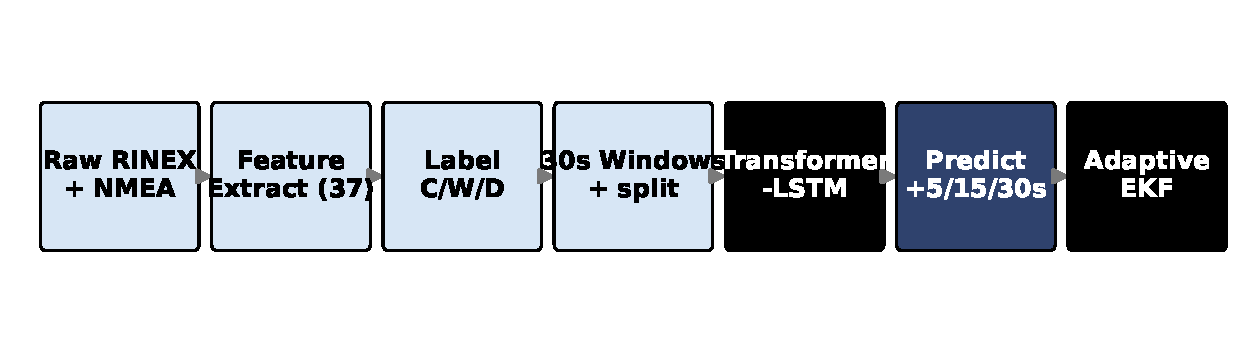
\includegraphics[width=0.9\columnwidth]{../../results/paper_figures/fig15_pipeline.pdf}
  \captionof{figure}{The full data pipeline from raw RINEX/NMEA to labelled
  feature windows — implemented by Joshua.}
\end{center}

\posec{Feature Engineering (37 features)}
\begin{poblock}
\begin{tabular}{lcp{4.5cm}}
  \toprule
  Group & \# & Key features \\
  \midrule
  Position quality & 4 & H/V error, PDOP, HDOP \\
  Signal strength & 8 & Mean C/N$_0$, per-SV stats \\
  Satellite geometry & 6 & SV count, elevation stats \\
  Pseudorange & 7 & Residuals, $\Delta$pseudorange \\
  Temporal & 5 & 10-s rolling mean/std \\
  Atmospheric & 4 & Tropo/iono delays \\
  Receiver status & 3 & \texttt{receiver\_tier}, lock time \\
  \bottomrule
\end{tabular}

\medskip
\textbf{Bug fixed:} Delta-pseudorange at session boundaries produced $\pm$500\,m
artifacts. Fixed with 3-point median filter. Affected $\approx$60 windows/session.
\end{poblock}

\posec{Dataset Assembly \& Labelling}
\begin{poblock}
\textbf{3-class labelling criteria:}
\begin{itemize}
  \item \textbf{CLEAN}: error $< 2$\,m AND C/N$_0 > 35$\,dB-Hz
  \item \textbf{DEGRADED}: error $> 5$\,m OR C/N$_0 < 30$ OR SV $< 4$
  \item \textbf{WARNING}: all other epochs
\end{itemize}

\textbf{Sliding window}: $(t-59, \ldots, t) \to$ predict at $t+5, t+15, t+30$

\textbf{Session-level split (70/15/15)} — prevents temporal leakage:
no epoch from a test drive appears in any training window.
\end{poblock}

\begin{center}
  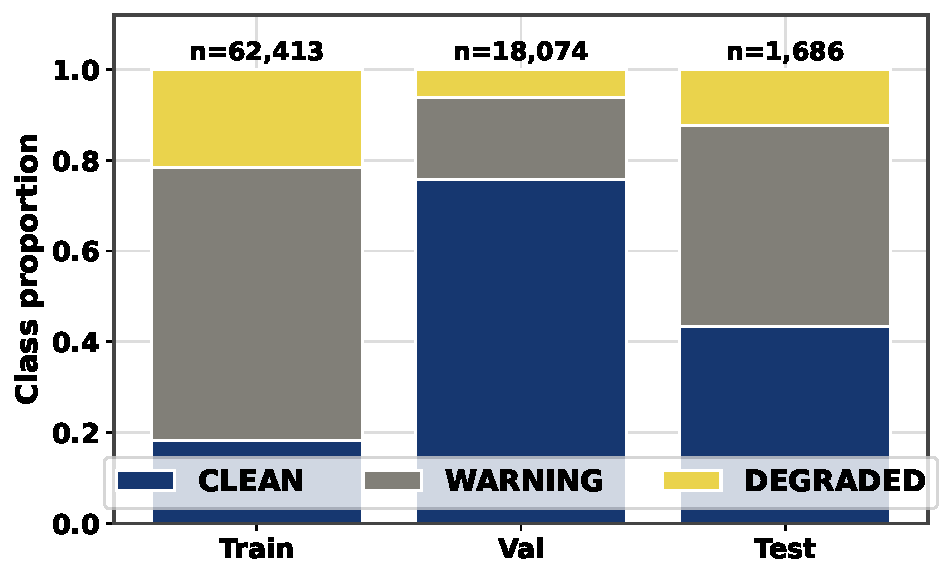
\includegraphics[width=0.9\columnwidth]{../../results/paper_figures/fig11_class_distribution.pdf}
  \captionof{figure}{Class distribution per split. DEGRADED: 7.8\,\% of training
  windows. Handled by focal loss + class weighting.}
\end{center}

\posec{Quality Assurance}
\begin{poblock}
Issues found and fixed:
\begin{enumerate}
  \item C/N$_0 = 0$ when SV count $> 0$: firmware artifact →
    imputed with session running mean
  \item Negative PDOP (RTKLIB extrapolation artifact) →
    clipped to minimum 1.0
  \item Delta-pseudorange boundary spikes → median filter
\end{enumerate}

\textbf{Leakage verification:}
\begin{itemize}
  \item Session IDs non-overlapping across splits ✓
  \item Scaler fit only on training data ✓
  \item \texttt{scenario\_a\_r13} within-site overlap disclosed ✓
\end{itemize}

After QA: \textbf{zero NaN rows} across all 149,662 windows.
\end{poblock}

\posec{Final Dataset Stats}
\begin{poblock}
\begin{tabular}{lccc}
  \toprule
  Split & Windows & CLEAN\,\% & DEG\,\% \\
  \midrule
  Train    & 104,763 & 58.2 & 7.8 \\
  Validate &  22,449 & 57.1 & 8.4 \\
  Test     &   1,686 & 43.4 & 12.4 \\
  \midrule
  \textbf{Total} & \textbf{149,662} & \multicolumn{2}{c}{4 cities · 9+ receivers} \\
  \bottomrule
\end{tabular}
\end{poblock}

\begin{center}
  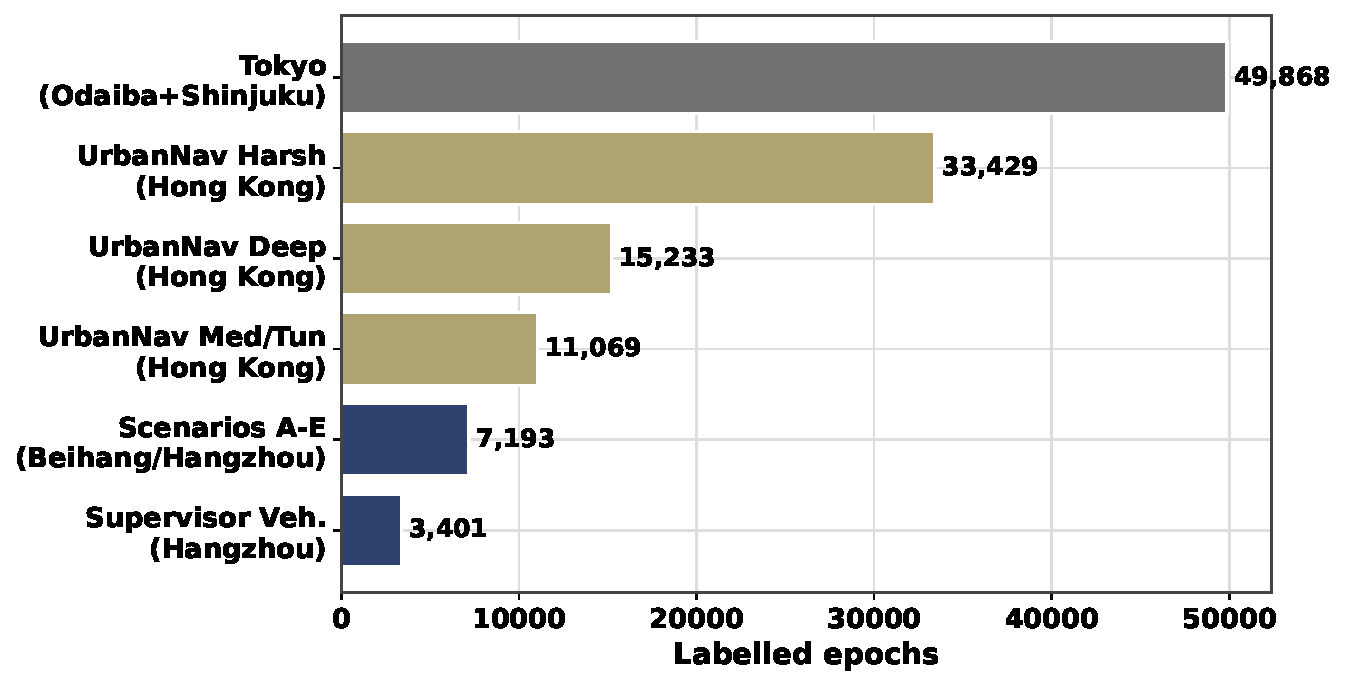
\includegraphics[width=0.9\columnwidth]{../../results/paper_figures/fig10_dataset_composition.pdf}
  \captionof{figure}{Dataset composition: most diverse labelled GNSS
  degradation benchmark known to us.}
\end{center}

\posec{Key Lesson}
\begin{poblock}
\textbf{Session-level split is essential for honest evaluation.}
A random 70/15/15 split mixes timesteps from the same drive between train and test,
artificially inflating metrics by 5–10\,\% because the model ``knows'' the transition
dynamics of each route.
Session-level splitting is the correct methodology for temporal sequence classification
in navigation datasets.
\end{poblock}

\end{multicols}

\noindent{\color{buaaBlue}\rule{\linewidth}{1.5pt}}\\[2pt]
{\small\color{buaaNavy}\centering Beihang University H3I · 2025}

\end{document}
